\documentclass[8pt]{extarticle}
% Font
\usepackage[default]{opensans}
\linespread{1.25}
% Margins
\usepackage[top=30mm,bottom=18mm,left=18mm,right=18mm]{geometry}
% Graphics and images
\usepackage{graphicx}
% Encodings (to render letters with diacritics and special characters)
\usepackage[utf8]{inputenc}
\usepackage[T1]{fontenc}
% Language
\usepackage[portuguese]{babel}
% Hyperreferences
\usepackage{hyperref}
\hypersetup{
    colorlinks=true,
    linkcolor=blue,
    filecolor=magenta,      
    urlcolor=blue,
}
\urlstyle{same}
% Headers and footers
\usepackage{fancyhdr}
\pagestyle{fancyplain}
\fancyhf{}
\lhead{Diogo Miguel Ferreira Rodrigues}
\rhead{\thepage}
% Subsections
\usepackage{titlesec}
\titleformat{\subsection}{\large}{\thesubsection}{}{\scshape}
\titlespacing*{\subsection}{0pt}{0pt}{0.6\baselineskip}
% Commands
%\usepackage{showframe}
%% Parag
\newcommand{\parag}[1]{
\begin{minipage}{\textwidth} \hfill
\begin{minipage}{\dimexpr\textwidth-0.6cm}
	#1
\end{minipage}
\end{minipage}
}
%% Itemtime
\newcommand{\itemtime}[2]{
#1 \hfill \begin{minipage}[t]{0.185\textwidth}         #2  \end{minipage}
}
%% Job
\newcommand{\job}[3]{\parag{
\itemtime{\textbf{#1}}{\textbf{#2}}\\
#3 \vspace*{9px}}}
%% Pub
\newcommand{\pub}[3]{\parag{
\itemtime{\textit{#1}}{#2}\\
#3 \vspace*{9px}}}
%% Idiom
\newcommand{\idiom}[2]{\textbf{#1} – #2\vspace*{6px}\\}
% Document
\begin{document}
\thispagestyle{empty}
\noindent
\begin{minipage}[l]{0.75\textwidth}
	\section*{Diogo Miguel Ferreira Rodrigues}
	Rua de Avioso, 553 | Castêlo da Maia (4475-617 MAIA)\\
    \href{mailto:diogo.rodrigues@fe.up.pt}{diogo.rodrigues@fe.up.pt}, \href{mailto:dmfrodrigues2000@gmail.com}{dmfrodrigues2000@gmail.com} | +351 915507239
\end{minipage}%
\write18{ wget https://drive.google.com/uc?id=1GlOkA6Zz44z9D6SBoXGkoN8oMophAt6o -O cv_photo.jpg ; }
\begin{minipage}[l]{0.24\textwidth}
	\begin{center} 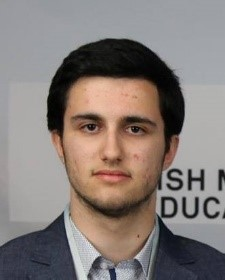
\includegraphics[scale=1]{cv_photo.jpg} \end{center}
\end{minipage}
\subsection*{Educação}
\job{Mestrado Integrado em Engenharia Informática e Computação}{2018 – 2023}{
Faculdade de Engenharia da Universidade do Porto\\
Colocado na 1ª fase, com classificação de ingresso 193.8/200.0\\
Conclusão do 1º ano com classificação 19.03/20.00
}
\job{Ensino Secundário – Curso Científico-Humanístico de Ciências e Tecnologias (10º-12º anos)}{2015 – 2018}{
Escola Secundária do Castêlo da Maia\\
Nível 3 de qualificação do Quadro Europeu de Qualificações\\
Conclusão com média 19.6/20.0\\
Exame Nacional de Matemática A (12º ano): 18.8/20.0\\
Exame Nacional de Física e Química A (11º ano): 19.5/20.0\\
Exame Nacional de Português (12º ano): 16.5/20.0\\
Exame Nacional de Biologia e Geologia (11º ano): 17.5/20.0\\
Disciplinas opcionais (12º ano): Física, Aplicações Informáticas B\\
Disciplinas específicas (10º/11º anos): Física e Química A, Biologia e Geologia\\
Membro do Quadro de Excelência nos anos letivos 2015/16, 2016/17 e 2017/18\\
Membro do Quadro de Mérito no ano letivo 2017/18\\
Prémio de Mérito do Ministério da Educação, por melhor classificação do estabelecimento escolar
}
\job{3º ciclo do Ensino Básico (7º-9º anos)}{2012 – 2015}{
Escola Básica do 2º e 3º Ciclos do Castêlo da Maia (EB2/3 Castêlo da Maia) – 7º ano\\
Escola Secundária do Castêlo da Maia (ESCM) – 8º/9º anos\\
Conclusão com média 5.0/5.0\\
Segunda língua estrangeira: Francês\\
Oferta de Escola (8º/9º): Oficina de Artes\\
Membro do Quadro de Excelência nos anos letivos 2012/13, 2013/14 e 2014/15
}
\job{2º ciclo do Ensino Básico (5º-6º anos)}{2010 – 2012}{
Escola Básica do 2º e 3º Ciclos do Castêlo da Maia (EB2/3 Castêlo da Maia)\\
Conclusão com média 5.0/5.0\\
Membro do Quadro de Excelência nos anos letivos 2010/11 e 2011/12
}
\job{1º ciclo do Ensino Básico (1º-4º anos)}{2006 – 2010}{
Escola Básica do 1º Ciclo/Jardim de Infância do Castêlo da Maia (EB1/JI Castêlo da Maia)
}
\subsection*{Cargos \& experiência}
\job{Assistente de Investigação}{2019 -}{
INESC-TEC – Laboratório de Inteligência Artificial e Apoio à Decisão (LIAAD)\\
\textit{Research on European Children and Adults Born Preterm} (RECAP)
}
\job{Membro do Comité Científico das \textit{Olimpíadas Nacionais de Informática – ONI}}{2018 – }{
Convidado na condição de ex-participante nas \textit{Olimpíadas Nacionais de Informática} e nas \\
\mbox{\textit{Olimpíadas Internacionais de Informática}}
}
\job{Representante dos alunos no Conselho Geral do Agrupamento de Escolas do Castêlo da Maia}{2017 – 2018}{
Agrupamento de Escolas do Castêlo da Maia\\
Mandato único alocado à Lista A, vencedora da eleição realizada em 18-10-2017
}
\subsection*{Competências}
\parag{
\textbf{Linguagens de programação:}\\
Nível avançado: C/C++, Python, Javascript, MATLAB, makefile\\
Nível intermédio: PHP, R, GNU Bash, SQL\\
Nível fundamental: Assembly (ARMv7, ARMv8), Visual Basic\\ 
\textbf{Tecnologias:}\\
Git: controlo de versões, branching, submódulos\\
Github: issues, projects, actions/workflows\\
Tecnologias web: NodeJS, cURL, pedidos HTTP por Ajax e XHR\\
\textbf{Outras competências:}\\
Elaboração de documentos em LaTeX e Markdown\\
Terminais Unix, GNU Bash shell\\
Sistemas operativos Linux (Ubuntu)
}
\subsection*{Publicações \& artigos}
\pub{AI Approach to Population Demographics using Satellite Imagery}{2019}{
\textit{London International Youth Science Forum 2019}\\
Apresentação financiada pela Fundação Calouste Gulbenkian
}
\subsection*{Bolsas}
\job{Bolseiro Gulbenkian}{24-07-2019 – 07-08-2019}{
Participação no \textit{London International Youth Science Forum 2019}\\
Imperial College London \& Royal Geographical Society, Londres\\
Apresentação de trabalho em formato poster\\
Participação financiada pela Fundação Calouste Gulbenkian
}
\subsection*{Voluntariado}
\job{\textit{European Union Science Olympiad 2019 – Almada}}{04-05-2019 – 11-05-2019}{
Guia das equipas \textit{Italy A} e \textit{Italy B} na \textit{European Union Science Olympiad 2019}, em Almada e Lisboa\\
Organização da EUSO e acompanhamento dos alunos participantes na competição durante a semana, garantindo o seu bem-estar e providenciar o apoio necessário aos alunos estrangeiros, nomeadamente na facilitação da sua estadia em Portugal com traduções para inglês e contextualização sociocultural durante os eventos.
}
\subsection*{Promoção da Ciência}
\job{Entrevista à RTP sobre a Medalha de Prata na \textit{EUSO2017}}{16-05-2017}{
Entrevista realizada a pedido da Rádio e Televisão de Portugal (RTP) no contexto da medalha de Prata\\
conquistada pela Equipa Portuguesa A que liderava na \textit{European Union Science Olympiad 2017 – Copenhagen}\\
\url{https://www.rtp.pt/noticias/pais/portugal-ganhou-medalha-de-prata-nas-olimpiadas-europeias-da-ciencia_v1001995}
}
\subsection*{Competições \& medalhas}
\job{\textit{Prémio Incentivo a estudantes distintos} da Universidade do Porto}{2018/19}{
Atribuído pela Universidade do Porto a estudantes distintos em primeiro ano de matrícula.\\
Pela obtenção da classificação média de 19.03/20.00 no final do 1º ano de curso\\
Melhor classificação da Faculdade de Engenharia da Universidade do Porto\\
2ª melhor classificação da Universidade do Porto
}
\job{Participação no \textit{SouthWestern Europe Regional Contest – SWERC2019-20}}{24-01-2020 – 27-01-2020}{
Institut Polytechnique de Paris, Paris, França\\
40º lugar na classificação geral
}
\job{1º lugar na \textit{Competição de Programação da Semana de Informática 2019}}{27-10-2019 – 30-10-2019}{
Faculdade de Engenharia da Universidade do Porto
}
\job{6º lugar na \textit{Maratona Inter-Universitária de Programação – MIUP2019}}{12-10-2019}{
Instituto Superior Técnico, Lisboa
}
\job{Participação no \textit{Google Code Jam}}{2019}{
Ronda de qualificação – 1093º; ronda 1A – 2738º; ronda 1B – 1848º; ronda 1C – 3897º
}
\job{Participação no \textit{Google Hash Code 2019}}{28-03-2019}{
\textit{Porto Hub} – Faculdade de Engenharia da Universidade do Porto\\
7º lugar no \textit{Porto Hub}, 31º a nível nacional, 2345º na classificação geral
}
\job{Prémio de \textit{Excelência Escolar 2017/2018}}{22-02-2019}{
Atribuído pela Câmara Municipal da Maia, no contexto da \textit{X Gala da Educação}
}
\job{Participação no \textit{SouthWestern Europe Regional Contest – SWERC2018} (\textit{ICPC2018})}{01-12-2018 – 02-12-2018}{
Télécom ParisTech, Paris, França\\
33º lugar na classificação geral
}
\job{1º lugar na \textit{Competição de Programação da Semana de Informática 2018}}{29-10-2018 – 01-11-2018}{
Faculdade de Engenharia da Universidade do Porto
}
\job{Medalha de Bronze na \textit{Maratona Inter-Universitária de Programação – MIUP2018}}{13-10-2018}{
Departamento de Informática da Universidade da Beira Interior, Covilhã\\
4º lugar na classificação geral
}
\job{Participação na \textit{30th International Olympiad in Informatics – IOI2018}}{01-09-2018 – 08-09-2018}{
Tsukuba, Ibaraki, Japão
}
\job{Menção Honrosa na \textit{49th International Physics Olympiad – IPhO2018}}{21-07-2018 – 29-07-2018}{
Lisboa, Portugal\\
2º lugar de entre os alunos portugueses, 226º na classificação global
}
\job{Medalha de Prata no \textit{Concurso Ibero-Americano de Informática e Computação – CIIC2018}}{09-06-2018}{
Departamento de Ciência de Computadores – Faculdade de Ciências da Universidade do Porto (para \\os alunos portugueses)
}
\job{7º lugar nacional na Final Nacional das \textit{Olimpíadas Nacionais de Informática – ONI2018}}{07-05-2018}{
Departamento de Ciência de Computadores – Faculdade de Ciências da Universidade do Porto\\
Convidado para participar no estágio de preparação para a \textit{International Olympiad in Informatics 2018}
}
\job{9º lugar no \textit{Mat12 2018}}{26-04-2018}{
Universidade de Aveiro – \textit{Competições Nacionais de Ciência} (CNC) \\
\textit{Mat12} – competição de matemática, categoria 12º ano
}
\job{3º lugar nacional na Fase de Qualificação das \textit{Olimpíadas Nacionais de Informática – ONI2018}}{12-04-2018 – 14-04-2018}{
Convite para participar na Final Nacional das \textit{Olimpíadas Nacionais de Informática 2018}
}
\job{Participação na Final Nacional das \textit{XXXVI Olimpíadas Portuguesas de Matemática}}{22-03-2018 – 25-03-2018}{
Agrupamento de Escolas de Mirandela, Mirandela\\
Categoria B (10º-12º anos)
}
\job{Medalha de Prata nas \textit{XLI Olimpíadas Paulistas de Matemática}}{28-10-2017}{
Departamento de Matemática da Universidade de Coimbra (para os alunos portugueses)\\
Categoria Gamma (11º/12º anos)
}
\job{Participação nas \textit{Olimpíadas Nacionais de Física 2017}}{02-06-2017 – 03-06-2017}{
Faculdade de Ciências da Universidade de Lisboa\\
Categoria B (até 11º ano)\\
Convite para integrar o Projeto Quark!
}
\job{Medalha de Prata na \textit{European Union Science Olympiad 2017 – Copenhagen}}{07-05-2017 – 14-05-2017}{
6º lugar na classificação global – Medalha de Prata\\
Provas realizadas na \textit{University of Copenhagen} e na \textit{Technical University of Denmark}
}
\job{Medalha de Ouro nas \textit{Olimpíadas Regionais de Física 2017 – Região Norte}}{29-04-2017}{
Departamento de Física e Astronomia – Faculdade de Ciências da Universidade do Porto\\
Categoria B (até 11º ano)\\
Convite para participar nas \textit{Olimpíadas Nacionais de Física 2017}
}
\job{Medalha de Bronze nas Semifinais das \textit{Olimpíadas de Química\textsuperscript{+} 2017}}{11-03-2017}{
Departamento de Química e Bioquímica – Faculdade de Ciências da Universidade do Porto\\
Categoria + (mais) (10º/11º anos)
}
\job{Participação nas \textit{XL Olimpíadas Paulistas de Matemática}}{19-11-2016}{
Departamento de Matemática da Universidade de Coimbra (para os alunos portugueses)\\
Categoria Gamma (11º/12º anos)
}
\job{11º lugar no \textit{Mat12 2016}}{11-05-2016}{
Universidade de Aveiro – \textit{Competições Nacionais de Ciência} (CNC) \\
\textit{Mat12} – competição de matemática, categoria 10º ano
}
\job{Medalha de Bronze nas \textit{XXXIX Olimpíadas Paulistas de Matemática}}{07-11-2015}{
Departamento de Matemática da Universidade de Coimbra (para os alunos portugueses)\\
Categoria Beta (9º/10º anos)
}
\job{Medalha de Ouro nas \textit{Olimpíadas Nacionais de Física 2015}}{05-06-2015 – 06-06-2015}{
Museu da Eletricidade (atualmente MAAT – Museu de Arte, Arquitetura e Tecnologia), Lisboa\\
Categoria A (até 9º ano)\\
Convite para participar na seleção para a \textit{European Union Science Olympiad 2017 – Copenhagen}
}
\job{19º lugar no \textit{Equamat 2015}}{13-05-2015}{
Universidade de Aveiro – \textit{Competições Nacionais de Ciência} (CNC) \\
\textit{Equamat} – competição de matemática, categoria 9º ano
}
\job{Participação nas \textit{XXI Olimpíadas de Maio}}{09-05-2015}{
Departamento de Matemática da Universidade de Coimbra (para os alunos portugueses)\\
Nível 2 (até 15 anos de idade)
}
\job{Medalha de Bronze nas \textit{Olimpíadas Regionais de Física 2015 – Região Norte}}{18-04-2015}{
Departamento de Física e Astronomia – Faculdade de Ciências da Universidade do Porto\\
Categoria A (até 9º ano)\\
Convite para participar nas \textit{Olimpíadas Nacionais de Física 2015}
}
\job{Participação na Semifinal das \textit{Olimpíadas de Química Júnior 2015}}{11-04-2015}{
Departamento de Química e Bioquímica – Faculdade de Ciências da Universidade do Porto\\
Categoria Júnior (8º/9º anos)
}
\job{Medalha de Bronze na Final Nacional das \textit{XXXIII Olimpíadas Portuguesas de Matemática}}{19-03-2015 – 22-03-2015}{
Escola Secundária Dr. Augusto César da Silva Ferreira, Rio Maior\\
Categoria A (8º/9º anos)\\
Convidado para participar no Projeto Delfos
}
\job{Participação nas \textit{XX Olimpíadas de Maio}}{10-05-2014}{
Departamento de Matemática da Universidade de Coimbra (para os alunos portugueses)\\
Nível 2 (até 15 anos de idade)
}
\job{12º lugar no \textit{Equamat 2014}}{29-04-2014}{
Universidade de Aveiro – \textit{Competições Nacionais de Ciência} (CNC) \\
\textit{Equamat} – competição de matemática, categoria 8º ano
}
\job{Medalha de Bronze nas \textit{XXXVII Olimpíadas Paulistas de Matemática}}{09-11-2013}{
Departamento de Matemática da Universidade de Coimbra (para os alunos portugueses)\\
Categoria Alpha (7º/8º anos)
}
\job{Participação nas \textit{XIX Olimpíadas de Maio}}{11-05-2013}{
Departamento de Matemática da Universidade de Coimbra (para os alunos portugueses)\\
Nível 1 (até 13 anos de idade)
}
\job{Participação no \textit{Desafio de Concepção e Corrida de Carrinhos Solares – À VELOCIDADE DO SOL}}{05-05-2013}{
Câmara Municipal da Maia
}
\job{Participação no \textit{Canguru Matemático sem Fronteiras 2013}}{04-04-2013}{
Prova realizada na Escola Básica de 2º e 3º Ciclos do Castêlo da Maia, Maia\\
Categoria Benjamim (7º/8º anos)
}
\job{Participação na Final Nacional das \textit{XXXI Olimpíadas Portuguesas de Matemática}}{14-03-2013 – 17-03-2013}{
Escola Básica de 2º e 3º Ciclos Dr. Francisco Cabrita, Albufeira\\
Categoria Júnior (6º/7º anos)
}
\job{1º lugar no concurso \textit{Problema do Mês}}{2011/2012}{
Realizado durante o ano letivo 2011/12 na Escola Básica de 2º e 3º Ciclos do Castêlo da Maia, Maia
}
\job{7º lugar no \textit{Canguru Matemático sem Fronteiras 2012}}{15-03-2012}{
Prova realizada na Escola Básica de 2º e 3º Ciclos do Castêlo da Maia, Maia\\
Categoria Escolar (5º/6º anos)\\
1º lugar a nível escolar, 7º lugar a nível nacional
}
\job{Participação no \textit{Canguru Matemático sem Fronteiras 2011}}{17-03-2011}{
Prova realizada na Escola Básica de 2º e 3º Ciclos do Castêlo da Maia, Maia\\
Categoria Escolar (5º/6º anos)
}
\subsection*{Fóruns, palestras, conferências \& congressos}
\job{\textit{Semana de Informática 2019}}{28-10-2019 – 31-10-2019}{
Faculdade de Engenharia da Universidade do Porto\\
Ciclo de palestras e \textit{workshops} organizado pelo Núcleo de Informática da AEFEUP
}
\job{\textit{London International Youth Science Forum 2019}}{24-07-2019 – 07-08-2019}{
Imperial College London \& Royal Geographical Society, Londres\\
Apresentação de trabalho em formato poster\\
Participação financiada pela Fundação Calouste Gulbenkian
}
\job{\textit{Evolução e Futuro da Inteligência Artificial – Repercussões Técnicas, Económicas, Sociais e Culturais}}{11-03-2019}{
Faculdade de Engenharia da Universidade do Porto\\
Seminário organizado no âmbito do ciclo \textit{Novos Paradigmas, Debates e Iniciativas na FEUP}
}
\job{\textit{Semana de Informática 2018}}{29-10-2018 – 01-11-2018}{
Faculdade de Engenharia da Universidade do Porto\\
Ciclo de palestras e \textit{workshops} organizado pelo Núcleo de Informática da AEFEUP
}
\job{Assembleia Municipal Jovem da Maia}{23-04-2018}{
Salão Nobre da Câmara Municipal da Maia\\
Realizada no contexto das Comemorações do 44º aniversário do 25 de abril de 1974\\
Deputado da Assembleia Municipal Jovem, em representação do Agrupamento de Escolas do Castêlo da Maia\\
Intervenção no Período de Antes da Ordem do Dia – Acessibilidade no concelho, e gestão de
resíduos sólidos urbanos
}
\job{\textit{CERN’s International Masterclasses Porto – 2018}}{10-03-2018}{
Departamento de Física e Astronomia – Faculdade de Ciências da Universidade do Porto\\
Percurso de palestras sobre física de partículas, análise de colisões de partículas no CERN e\\
discussão dos resultados com outros centros europeus e cientistas do CERN
}
\subsection*{Intercâmbios}
\job{Intercâmbio entre a Escola Secundária do Castêlo da Maia e a \textit{Rejsby Europæiske Efterskole}}{}{
\textit{Rejsby Europæiske Efterskole} – Ribe, Região da Dinamarca do Sul\\
\itemtime{Estadia na Dinamarca:}{17-02-2015 – 24-02-2015}\\
\itemtime{Acolhimento dos alunos dinamarqueses em Portugal:}{15-04-2015 – 22-04-2015}\\
}
\subsection*{Idiomas}
\parag{
\idiom{Português}{idioma nativo}
\idiom{Inglês}{falante fluente (C1), proficiente na leitura (C1) e escrita (C1) sobre assuntos complexos\\
\itemtime{
\textit{[Cambridge English Level 1 Certificate in ESOL International (Preliminary):\\
Pass with Distinction in the Preliminary English Test;\\
demonstrates an ability at Level 1 (UK National Qualifications Framework) and Council of Europe Level B2]}
}{27-07-2015}}
\idiom{Espanhol}{intermédio na fala (B2), leitura (B2) e escrita (B1)}
\idiom{Francês}{falante elementar (A2), intermédio na leitura (B2) e escrita (B1)}
}
\subsection*{Associações \& projetos}
\job{\textit{Research on European Children and Adults Born Preterm} (RECAP)}{Set/2018 – Mar/2019}{
O objetivo do projeto RECAP Preterm é melhorar a saúde, o desenvolvimento e a qualidade de vida de crianças e adultos nascidos prematuros na União Europeia, através do desenvolvimento da \textit{RECAP Preterm Cohort Platform}, uma base de dados sustentável, geograficamente diversa e multidisciplinar de \textit{cohorts} nacionais e Europeus de bebés muito prematuros ou com peso à nascença muito baixo, constituídos ao longo de 30 anos e desenhados de forma a otimizar a utilização de dados populacionais para investigação e inovação nas áreas da saúde, social e de educação.\\
Encontro-me a desenvolver uma aplicação web integrada no sítio web do projeto, que permita a realização de análises estatísticas de forma rápida e sem necessidade de conhecimentos sobre o funcionamento das ferramentas de acesso à base de dados, e apresentação de resultados de forma gráfica. Para isso estão a ser utilizadas as tecnologias NodeJS e DATAShield, e as linguagens JavaScript e R.
}
\job{Comunidade FEUP-SWERC}{2018 – }{
Comunidade colaborativa de alunos e professores da Faculdade de Engenharia da Universidade do Porto, com o objetivo de disseminar o gosto pela programação competitiva na comunidade FEUP, dinamizar competições de programação e selecionar/preparar os alunos da Faculdade para representação em competições de programação nacionais, europeias e internacionais.
}
\job{Orçamento Participativo das Escolas – Proposta \textit{UPAC-AECM}}{2018}{
Segundo proponente da Proposta UPAC-AECM, que consiste na instalação de uma Unidade de Produção e Autoconsumo (UPAC), constituída por um conjunto de painéis solares fotovoltaicos, na Escola Secundária do Castêlo da Maia. Proposta vencedora da eleição realizada em 23-03-2018, por maioria absoluta (50.3\% dos votos válidos).
}
\job{Projeto Quark!}{2018}{
Escola de excelência de Física para alunos dos 11º e 12º anos, com um processo de seleção altamente competitivo. Decorre no Departamento de Física da Universidade de Coimbra, aos fins-de-semana. Membro do grupo dos 19 pré-selecionados para as competições internacionais (através das Olimpíadas Nacionais de Física 2017). \textbf{1º lugar} nas Provas de Seleção/Apuramento para as Provas Internacionais (“Provas de Fogo” – PDF) realizadas em 19-05-2018, apurando-se para a \textbf{\textit{49th International Physics Olympiad – IPhO2018}}, em Lisboa, Portugal.
}
\job{Projeto Delfos}{2013; 2015 – 2016}{
Projeto de Matemática com o objetivo de preparar os representantes portugueses em competições internacionais de Matemática. Decorre no Departamento de Matemática da Universidade de Coimbra, aos fins-de-semana.
}
\end{document}
